\section{Rearraning Calculations}\label{sec:2}
The number of calculations is now split into $P = \num{100}$ and
$X = \num{100}$. In this case we get a value of
\begin{equation}
	\pi_f = \num{3.15 \pm 0.16}.
\end{equation}
This value has a much smaller error (\per{5.1}) compared to \cref{sec:1}. A histogram 
for the distribution of $\pi_x$ is shown in \cref{fig:pi_hist_100_100}.
With $P=1$ and $X = \num{10000}$ we get a value of 
\begin{equation}
    \pi_f = \num{3.2\pm 1.7},
\end{equation}
which is identical to the calculation from \cref{sec:1}.

\begin{figure}[h!]
	\centering
	\begin{minipage}{0.45\linewidth}
		\centering
		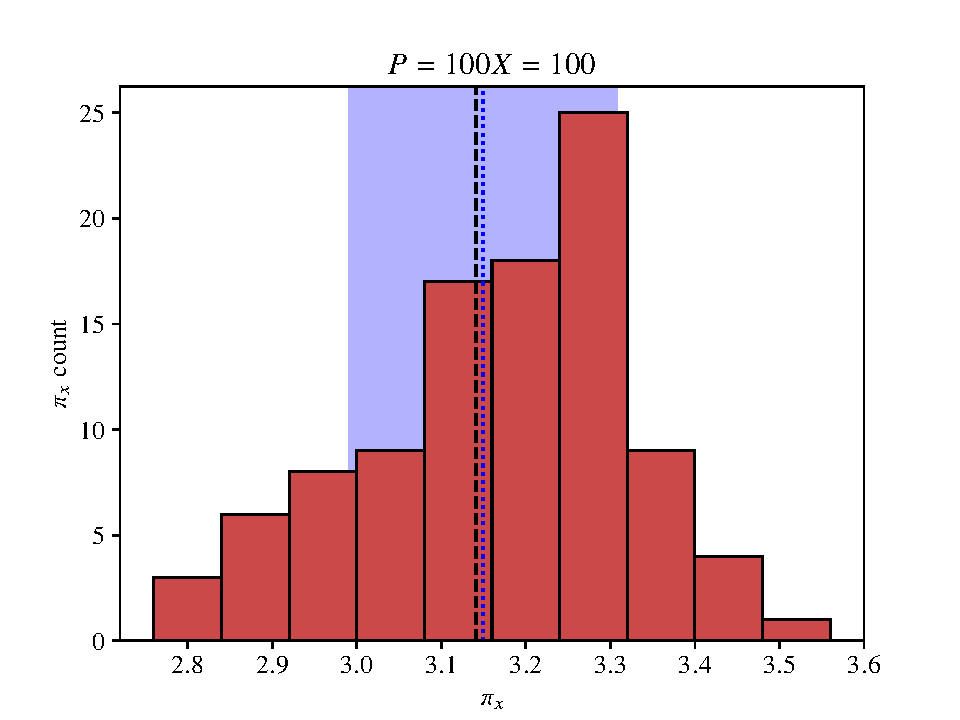
\includegraphics[width=\linewidth]{figs/ex1.2_pi_hist_100_100.pdf}
		\caption{Histogram of calculated $\pi$ values with $P = 100$ and
			$X = 100$.}
		\label{fig:pi_hist_100_100}
	\end{minipage}
    \hfill
    \begin{minipage}{.45\linewidth}
       \centering
       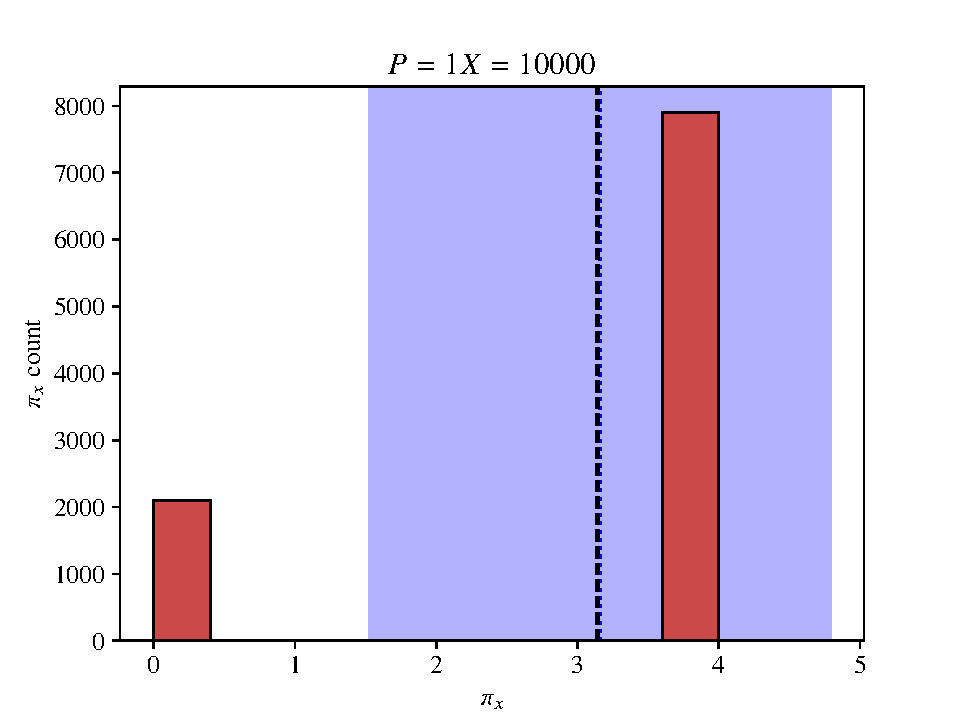
\includegraphics[width=\linewidth]{figs/ex1.2_pi_hist_1_10000.pdf} 
		\caption{Histogram of calculated $\pi$ values with $P = 1$ and
			$X = \num{10000}$.}
		\label{fig:pi_hist_1_10000}
    \end{minipage}
\end{figure}







